\documentclass[conference]{IEEEtran}
\IEEEoverridecommandlockouts

\usepackage[utf8]{inputenc}
\usepackage{cite}
\usepackage{amsmath,amssymb,amsfonts}
\usepackage{algorithmic}
\usepackage{graphicx}
\usepackage{textcomp}
\usepackage{xcolor}
\usepackage{bytefield}
\usepackage{url}
\usepackage[whole]{bxcjkjatype}

\def\BibTeX{{\rm B\kern-.05em{\sc i\kern-.025em b}\kern-.08em
    T\kern-.1667em\lower.7ex\hbox{E}\kern-.125emX}}
\begin{document}

\title{Adaptive Source Routing in SRv6 using Programmable SRv6 Functions and eBPF}

\author{\IEEEauthorblockN{Yuzuki Ishiyama (ID:2531008)}
  \IEEEauthorblockA{\textit{Yamaki Laboratory} - \textit{Information and Network Engineering}}
}

\maketitle

\begin{abstract}
  Segment Routing over IPv6 (SRv6) is gaining attention as a flexible routing mechanism to meet the diverse requirements of modern networks.
  However, SRv6 has inherent limitations. Since routing decisions are made statically at the source, it is impossible to adapt to network conditions that change after packet transmission.
  This research proposes a novel method to achieve adaptive source routing using SRv6 Functions.
  By directly encoding path branching conditions into the segment list, this method enables dynamic path selection based on real-time network metrics without relying on additional control packets.
  We implemented this method on Linux routers using eBPF and demonstrated its feasibility through experimental evaluation.
  Compared to conventional probe-based methods, our approach showed 43.1\% higher throughput and more stable network performance.
  The throughput reduction due to overhead was 1.04%.
\end{abstract}

\begin{IEEEkeywords}
  service function chaining, segment routing, SRv6, QoS
\end{IEEEkeywords}

\section{Introduction}

Internet Service Providers (ISPs) are increasingly adopting source routing technologies to implement diverse routing policies for various applications \cite{cisco_rakuten_srv6}\cite{softbank_srv6}.
Source routing, where the source specifies the path a packet should take, offers improved scalability and controllability compared to traditional hop-by-hop forwarding.
Segment Routing over IPv6 (SRv6) is a protocol that implements source routing by embedding path information in an IPv6 extension header.
SRv6 is widely adopted due to its ease of deployment in IPv6 networks compared to other technologies.

However, source routing has a fundamental limitation: path decisions must be made when a packet is sent, making it unable to adapt to network conditions that change after transmission.
This research proposes a method to overcome this limitation by directly encoding path branching conditions into the SRv6 segment list.
This approach enables dynamic path selection based on real-time network metrics without requiring additional control messages.

\section{Background}

\subsection{Source Routing and Potential Issues}

Traditional IP routing faces challenges in implementing complex routing policies.
This is because each router refers only to the destination address in the packet header and independently determines the next hop based on its own routing table.
Consequently, intermediate routers cannot perform path selection that considers application requirements or end-to-end path characteristics.

Source routing addresses the aforementioned problems, allowing the sender to specify the complete path a packet should traverse through the network.
This paradigm provides application-specific routing with scalability and flexibility. SRv6 implements source routing by adding a Segment Routing Header (SRH) to IPv6 packets \cite{rfc8754}\cite{rfc9256}.
The SRH contains a segment list, which is a sequence of Segment Identifiers (SIDs) representing the nodes to be traversed.
In most cases, SIDs are IPv6 addresses.

However, source routing has a fundamental limitation.
Routing decisions are made statically at the source, making it impossible to adapt to network conditions that change after packet transmission.

\subsection{SRv6 Function}

The segment list can also include function calls.
This function, called an SRv6 Function, is an instruction that specifies an operation to be performed when a packet reaches a specific node.
Each instruction is encoded in the format of an IPv6 address and consists of three parts: Locator, Function, and Arguments.
% Figure \ref{fig:example-of-dividing-an-ipv6-address} shows the structure of an IPv6 address.
The Locator points to the node where the Function is executed, and the Function and Arguments specify the operation to be performed at that node.

% show locator, function, and arguments in a bytefield
% | 128 bits                       |
% | 64 bits | 16 bits  | 48 bits   |
% | Locator | Function | Arguments |

% \begin{figure}[htbp]
%   \centering
%   \begin{bytefield}[bitwidth=0.18em]{128}
%     \bitheader{0, 16, 32, 48, 64, 80, 96, 112, 128} \\
%     \bitbox{64}{\small LOC} & \bitbox{16}{\small FUNC} & \bitbox{48}{\small ARG} \\
%   \end{bytefield}
%   \caption{Example of dividing an IPv6 address}
%   \label{fig:example-of-dividing-an-ipv6-address}
% \end{figure}

\section{Proposed Method}
% \subsection{Encoding Conditions in SRv6 Function}

The basic concept is to include branching conditions based on network metrics and their corresponding paths in the segment list.

To implement conditional paths in the segment list, we define two SRv6 Functions: \textit{skip\_if} and \textit{skip}.
\textit{skip\_if} skips a specified number of subsequent segments based on a metric condition, such as bandwidth.
\textit{skip} simply skips a specified number of subsequent segments.
For example, if a condition $condition$ (e.g., the bandwidth between router A and B exceeds a threshold) is true, forward to router C, otherwise forward to router B, the segment list would be $\{ \text{A:\textit{skip\_if}}(1, condition), \text{B:\textit{skip}}(1), \text{C} \}$.

% [Below text] Priority: Low
% To reduce noise in metric measurements, metrics are smoothed using an Exponential Moving Average (EMA).
% The EMA is calculated by the following formula:
% \begin{equation}
%   \text{EMA}_t = \alpha \cdot x_t + (1 - \alpha) \cdot \text{EMA}_{t-1}
% \end{equation}
% where \(x_t\) is the current measurement, \(\text{EMA}_{t-1}\) is the previous EMA value, and \(\alpha\) is the smoothing factor.

\section{Evaluation Setup}

\begin{figure}[t]
  \centering
  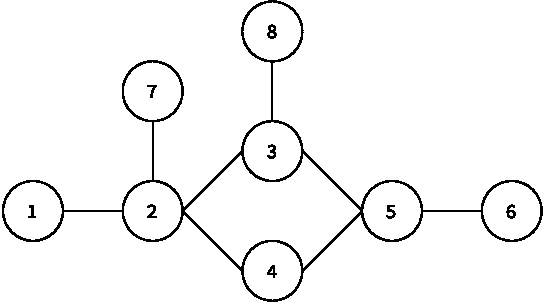
\includegraphics[width=0.7\linewidth]{./figures/topo.pdf}
  \caption{Network Topology}
  \label{fig:network-topology}
\end{figure}


% == OLD START ==
% We evaluated our method using a network topology with multiple potential paths between source and destination nodes. The Linux routers ran our eBPF implementation, and network namespaces, one of the linux features, are used for virtualization, tc for bandwidth/delay control, and iperf3 for traffic generation.
% The proposed method was evaluated using two scenarios:
% \begin{itemize}
%   \item \textbf{Scenario 1}: A single TCP flow that exceeds the threshold, requiring path switching.
%   \item \textbf{Scenario 2}: Two TCP flows competing for bandwidth, with dynamic path selection.
% \end{itemize}
% For comparison, the probe-based approach was also implemented using a separate control packet to probe the network condition.
% == OLD END ==

We evaluated our proposed method in terms of network quality and overhead.

The network quality evaluation was conducted using two scenarios in the network topology shown in Figure \ref{fig:network-topology}.
Each circle represents a router. A delay of 2 ms was set between router 1-2, and a bandwidth limit of 1 Gbps was set between router 2-3 and router 2-4.
In the first scenario, TCP communication is performed from router 1 to router 6.
Packets normally reach router 6 via routers 2, 3, and 5. However, if the bandwidth between router 2-3 exceeds 900 Mbps, the segment list is set so that the excess traffic reaches router 6 via router 4.
In the second scenario, the TCP communication between router 1-6 and the branching conditions are the same, but an additional TCP communication is performed from router 7 to router 8, causing the threshold to be exceeded by the additional TCP flow.
For comparison, a conventional probe-based method was also implemented. This uses a separate control packet to probe the network condition.

The overhead evaluation was performed by comparing TCP throughput with and without SRv6 Functions in the segment list.

\section{Evaluation Results}

% == OLD START ==
% In Scenario 1, the proposed method achieved 43.1\% higher throughput compared to the conventional probe-based approach.
% The performance improvement was attributed to the immediate path switching based on real-time metrics, which avoids TCP congestion control.
% In Scenario 2, our method maintained more stable bandwidth utilization across flows compared to the probe-based approach.
% The implementation overhead was minimal:
% \begin{itemize}
%   \item Protocol size increase: 3.2\%
%   \item Throughput reduction due to eBPF execution: 1.04\%
% \end{itemize}
% == OLD END ==

The evaluation results regarding network quality are shown.
In Scenario 1, the proposed method achieved 43.1\% higher throughput compared to the conventional method (Figure \ref{fig:scenario-1}).
In Scenario 2, the proposed method achieved more stable throughput compared to the conventional method (Figure \ref{fig:scenario-2}).
Note that the period from 20 seconds to 40 seconds is when TCP communication was performed between router 7-8.

In the overhead evaluation, when SRv6 Functions were included in the segment list, TCP throughput decreased by 1.04\% compared to when they were not included.

% == OLD START ==
% We proposed and implemented an adaptive source routing method using SRv6 Functions that enables dynamic path selection based on real-time network metrics.
% By encoding conditional logic directly into the Segment List, each router can make forwarding decisions based on the current network conditions.
% Experimental results demonstrated higher throughput and more stable performance compared to a conventional probe-based approach with minimal overhead.
% Future work includes supporting additional metrics and more complex conditions.
% == OLD END ==

\section{Discussion}

The proposed method presents a novel approach to achieving adaptive source routing by leveraging SRv6 Functions and directly embedding path branching conditions within the segment list.
The results of the evaluation experiments showed that this method achieved remarkable improvements in both network throughput and stability compared to conventional probe-based methods.
In particular, the 43.1\% throughput improvement observed in Scenario 1 is attributed to the proposed method's ability to detect network state changes in real-time and immediately optimize paths. This avoids the delays in state detection and the resulting inefficient operation of TCP congestion control mechanisms seen in conventional methods.
Similarly, the improvement in throughput stability in Scenario 2 is also considered to be due to this rapid adaptation capability.
In terms of implementation, the execution overhead of this method using eBPF was very small, with a throughput reduction of 1.04\%, and the increase in protocol header size was also limited.
While this study primarily used bandwidth as the decision criterion, the realization of more complex conditional branching logic combining various network metrics such as delay, jitter, and packet loss rate is expected in the future.

\begin{figure}[t]
  \centering
  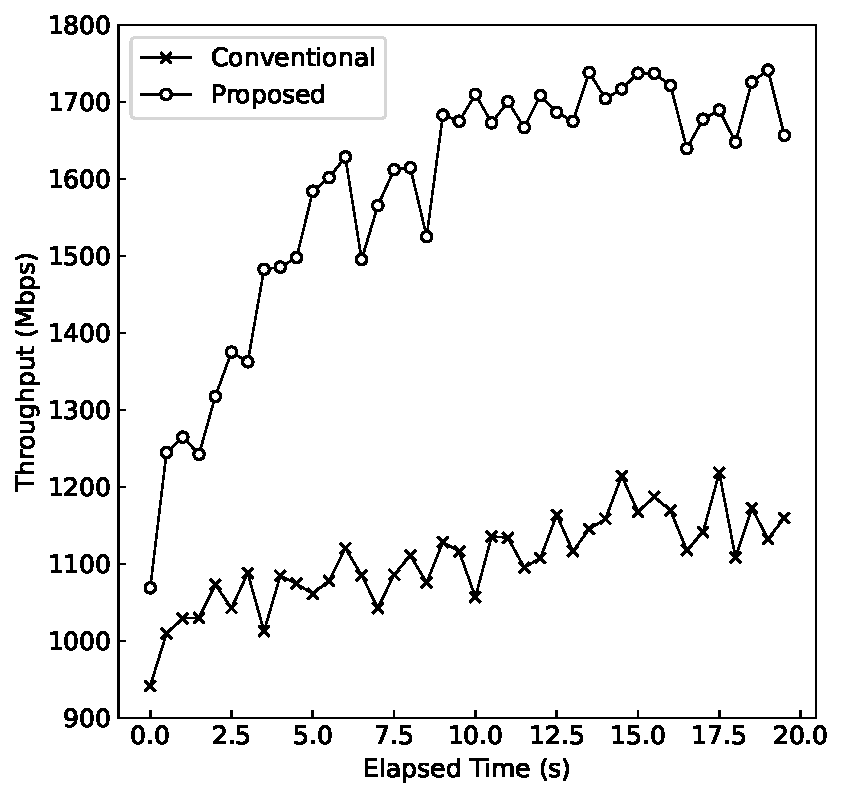
\includegraphics[width=0.7\linewidth]{./figures/scenario-1.pdf}
  \caption{Scenario 1: TCP Throughput}
  \label{fig:scenario-1}
\end{figure}

\begin{figure}[t]
  \centering
  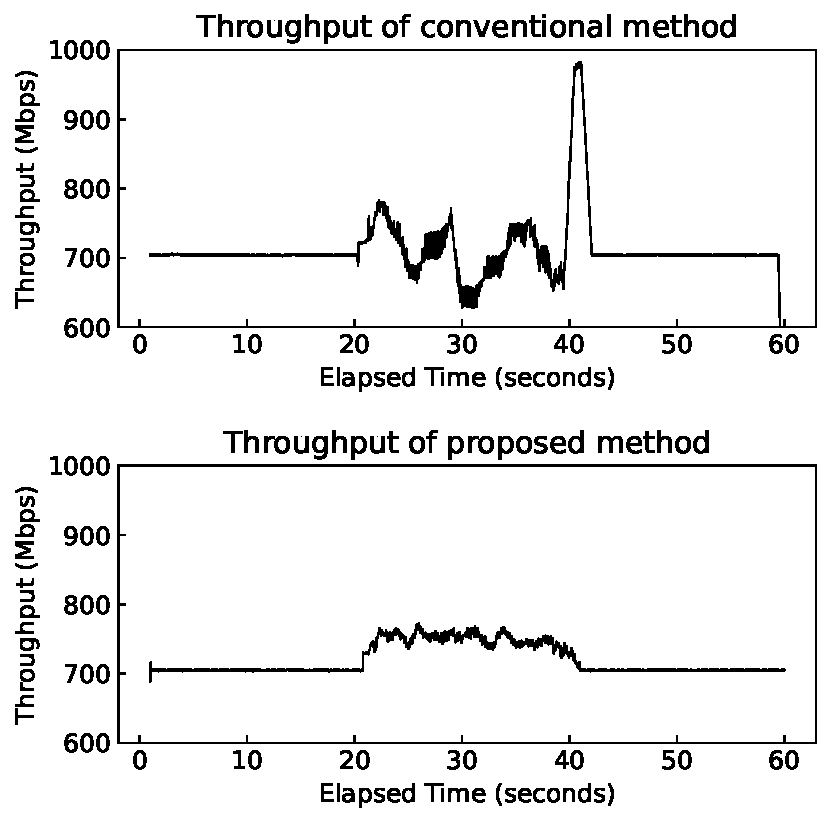
\includegraphics[width=0.7\linewidth]{./figures/scenario-2.pdf}
  \caption{Scenario 2: TCP Throughput}
  \label{fig:scenario-2}
\end{figure}

\section{Conclusion}

In this research, we proposed a novel method for achieving adaptive source routing using SRv6 Functions.
This method enables dynamic path selection based on real-time network metrics without relying on additional control packets by directly encoding path branching conditions into the segment list.
We implemented this method on Linux routers using eBPF and demonstrated its feasibility through experimental evaluation.
Compared to conventional probe-based methods, our approach showed higher throughput and more stable network performance.
The implementation overhead was minimal.
Future work includes supporting additional metrics and more complex conditions.

\bibliographystyle{IEEEtran}
\bibliography{refs}

\end{document}
